\chapter{Richiami di Termodinamica}
La Termodinamica studia sistemi macroscopici, senza preoccuparsi della loro struttura microscopica, tramite una manciata di variabili termodinamiche. La teoria si basa su quattro postulati che vengono giustificati a posteriori grazie al successo della Termodinamica nel descrivere i sistemi che intende studiare. Anche se i possibili sistemi oggetto della Termodinamica sono molteplici, tutti sono accomunati dalle equazioni che li descrivono, queste sono le equazioni di stato, derivate sperimentalmente e che hanno la caratteristica di legare le variabili termodinamiche tra di loro. Normalmente, l'obiettivo della Termodinamica è quello di ricavare l'equazione di stato, ossia le proprietà termodinamiche, del sistema macroscopico. Il primo ostacolo che si presenta è il fatto che i sistemi termodinamici macroscopici sono costituiti da un numero $N$ di componenti molto elevato, ad esempio, una singola mole di sostanza possiede $N_A$ componenti. Per questo motivo è impraticabile l'utilizzo sia di un approccio classico tramite la Meccanica newtoniana che di un approccio quantistico tentando di associare ad ogni componente la sua equazione di Schr\"odinger. Diventa quindi evidente la necessità di applicare un approccio basato su metodi statistici. Gli stati di equilibrio di un sistema sono determinati dalle variabili di stato, funzioni della temperatura $T$, della pressione $p$ e del volume $V$. Le variabili di stato si dividono in due classi:
\begin{enumerate}
    \item estensive, ossia grandezze che dipendono dalle dimensioni del sistema;
    \item intensive, ossia grandezze che non dipendono dalle dimensioni del sistema.
\end{enumerate}
A loro volta, i sistemi termodinamici si distinguono in:
\begin{enumerate}
    \item aperti, cioè che possono scambiare materia con l'ambiente;
    \item chiusi, cioè che non possono scambiare materia con l'ambiente;
    \item non isolati, cioè che possono scambiare energia con l'ambiente;
    \item isolati, cioè che non possono scambiare energia con l'ambiente.
\end{enumerate}
A seguito di una variazione della variabili termodinamiche o delle condizioni esterne, un sistema può passare da uno stato di equilibrio $A$ ad un altro stato di equilibrio $B$. Le trasformazioni che collegano questi due stati possono essere:
\begin{enumerate}
    \item reversibili, ovvero tali che in ogni istante le variabili di stato sono ben definite e che quindi, in linea di principio, si può invertire la trasformazione senza modificare l'ambiente esterno;
    \item irreversibili, ovvero tali che per invertire la trasformazione è necessario modificare l'ambiente esterno.
\end{enumerate}
Le trasformazioni reversibili sono ideali ma tendono ad approssimare le trasformazioni quasi statiche, mentre quelle irreversibili descrivono processi più generici dato che le trasformazioni reali tendono appunto ad essere, almeno in parte, irreversibili. In linea generale, il lavoro compiuto dal sistema $\delta W$ è dato da 
\begin{equation}
\label{eq: lavoro compiuto dal sistema}
    \delta W = pdV - \mu dN - ydX,
\end{equation}
dove $\mu$ è il potenziale chimico, $y$ sono le forze generalizzate e $dX$ sono gli spostamenti generalizzati. Quindi, in \eqref{eq: lavoro compiuto dal sistema} il termine $\mu dN$ corrisponde al lavoro compiuto per modificare il numero di componenti del sistema, mentre $ydX$ include tutti gli altri possibili processi che coinvolgono un certo lavoro da parte del sistema per essere compiuti. In particolare, il potenziale chimico svolge un ruolo analogo a quello della temperatura, infatti due sistemi $A$ e $B$ sono in equilibrio chimico se $\mu_A=\mu_B$. Inoltre, se un sistema è composto da un numero $i$ di sottosistemi caratterizzati da un potenziale $\mu_i$ e un numero di componenti $N_i$, allora 
\begin{equation}
\label{eq: contributo lavoro chimico sistema composto}
    \mu dN=\nsum_i\mu_idN_i.
\end{equation}
\begin{axiom}[principio 0 della Termodinamica]
\label{axiom: principio 0 della TD}
    Esiste una funzione di stato $T$ tale che due sistemi $A$ e $B$ sono in equilibrio energetico se $T_A=T_B$.
\end{axiom}
La funzione di stato $T$ che compare nel principio \ref{axiom: principio 0 della TD} è normalmente la temperatura $T$, inoltre dal medesimo si può derivare il seguente corollario.
\begin{corl}[equilibrio termico]
\label{corl: equilibrio termico a 3 corpi}
    Se un sistema $A$ è in equilibrio termico con un sistema $C$ e se un sistema $B$ è anch'esso in equilibrio termico con $C$, allora $A$ è in equilibrio termico con $B$.
\end{corl}
Dal corollario \ref{corl: equilibrio termico a 3 corpi} si possono definire i termometri e le scale empiriche di temperatura, in particolare tramite un termometro a gas perfetto si può definire una scala di temperatura assoluta, i Kelvin, dove $T = 0$ è la temperatura del gas a $p = 0$.
\begin{axiom}[I principio della Termodinamica]
\label{axiom: I principio della TD}
    Dato un sistema immerso in un ambiente, una variazione di energia $dE$ può avvenire solo tramite il bordo del sistema e corrisponde alla differenza tra il lavoro assorbito e compiuto dal sistema, per cui
    \begin{equation}
    \label{eq: I principio della TD}
        dE=\delta Q - \delta W.
    \end{equation}
\end{axiom}
Sostituendo l'espressione del lavoro \eqref{eq: lavoro compiuto dal sistema} nell'equazione \eqref{eq: I principio della TD} si ottiene la relazione 
\begin{equation}
\label{eq: combinazione espressione lavoro e I PDT}
    dE = \delta Q - pdV + \mu dN + ydx.
\end{equation}
Per quanto riguarda il secondo principio della Termodinamica, ne esistono due versioni equivalenti formulate rispettivamente da Celsius e da Kelvin.
\begin{axiom}[II principio della Termodinamica, Clausius]
\label{axiom: II principio della TD, Clausius}
    Dati due sistemi $A$ e $B$ di temperatura $T_A$ e $T_B$ rispettivamente, se $T_A>T_B$, allora il calore viene trasferito da $A$ a $B$ e non esiste alcuna trasformazione il cui unico effetto sia il trasferimento di calore da $B$ ad $A$.
\end{axiom}
\begin{axiom}[II principio della Termodinamica, Kelvin]
\label{axiom: II principio della TD, Kelvin}
    Dati due sistemi $A$ e $B$ di temperatura $T_A$ e $T_B$ rispettivamente, non esiste alcuna trasformazione il cui unico effetto sia la conversione in lavoro di tutto il calore prelevato da un'unica sorgente.
\end{axiom}
Si consideri ora una macchina ciclica reversibile, come quella in figura \ref{fig: macchina di Carnot 1}, che lavora tra due sorgenti a temperatura costante $T_2$ e $T_1$ rispettivamente, che assorbe il calore $Q_2$ da $T_2$, che compie il lavoro $W$ e che cede il calore $Q_1$ a $T_1$, con $T_2 > T_1$.
\begin{figure}[h]
    \centering
    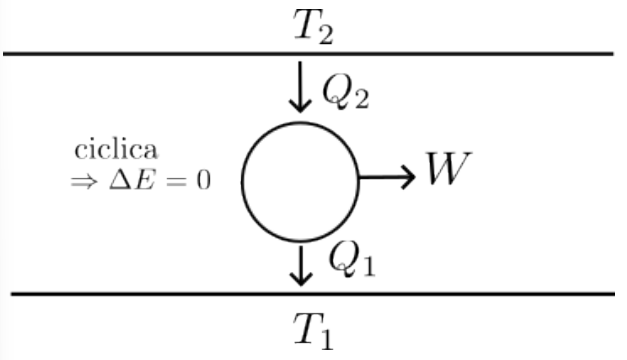
\includegraphics[width=0.4\linewidth]{Immagini/macchina di Carnot 1.png}
    \caption{macchina ciclica reversibile con $T_2 > T_1$.}
    \label{fig: macchina di Carnot 1}
\end{figure}

Per il secondo principio della Termodinamica (\ref{axiom: I principio della TD}), dato che la variazione di energia di una macchina ciclica è $\Delta E = 0$, il lavoro $W$ coincide con $W = Q_2 - Q_1$, per cui il rendimento $\eta$ della macchina in questione è
\begin{equation}
\label{eq: rendimento macchina ciclica reversibile}
    \eta = \frac{W}{Q_2} = \frac{Q_2 - Q_1}{Q_2} = 1 - \frac{Q_1}{Q_2} < 1,
\end{equation}
dove $Q_1 > 0$ per il primo principio della Termodinamica (\ref{axiom: II principio della TD, Clausius}). Un teorema fondamentale in Termodinamica, equivalente al secondo principio della Termodinamica, è il seguente.
\begin{teo}[di Carnot]
\label{teo: teorema di Carnot}
    Indicando con $R$ una generica macchina reversibile e con $I$ una generica macchina irreversibile, allora:
    \begin{enumerate}
        \item tutte le macchine termiche reversibili che utilizzano due sole sorgenti rispettivamente a temperatura $T_1$ e $T_2$ tali che $T_2 > T_1$, hanno lo stesso rendimento $\eta_R$ pari a quello di una macchina di Carnot che opera tra la medesima coppia di sorgenti, ovvero $\eta_R = \eta_C$;
        \item le macchine termiche irreversibili che utilizzano due sole sorgenti rispettivamente a temperatura $T_1$ e $T_2$ tali che $T_2 > T_1$, hanno un rendimento $\eta_I$ sempre minore di una macchina reversibile che opera tra la medesima coppia di sorgenti, ovvero $\eta_I < \eta_R$.
    \end{enumerate}
\end{teo}
La dimostrazione del teorema \ref{teo: teorema di Carnot} procede per assurdo ma si omette in questa sede. Dallo stesso segue che $\eta_R$ è lo stesso per tutte le macchine reversibili operanti tra $T_2$ e $T_1$, per cui
\begin{equation}
\label{eq: rapporto calori macchina reversibile}
    \frac{Q_{1R}}{Q_{2R}}=f(T_2,T_1),
\end{equation}
ossia il rapporto tra il calore assorbito e ceduto da una macchina reversibile deve essere esprimibile come una funzione dipendente solo dalla temperature delle sorgenti.

Fino ad ora si è dato per scontato che la scala della temperatura fosse quella assoluta $T$. Tuttavia, in linea di principio, si può utilizzare qualsiasi scala di temperatura $t$. A partire da questo, si può ottenere univocamente una temperatura termodinamica sfruttando le proprietà dei cicli di Carnot.
\begin{figure}[h]
    \centering
    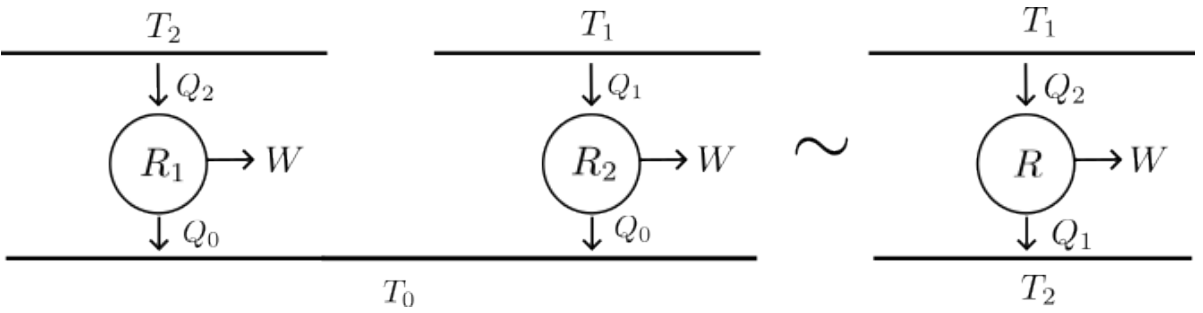
\includegraphics[width=0.8\linewidth]{Immagini/coppia macchine di Carnot.png}
    \caption{combinazione di due macchine cicliche reversibili.}
    \label{fig: coppia macchine di Carnot}
\end{figure}
Quindi, combinando due cicli di Carnot $R_1$ ed $R_2$, il primo operante tra $t_2$ e $t_0$, mentre il secondo tra $t_1$ e $t_0$, se ne può ottenere un  terzo operante tra $t_2$ e $t_1$, come mostrato in figura \ref{fig: coppia macchine di Carnot}. In base alla \eqref{eq: rapporto calori macchina reversibile}, si ha
\begin{equation}
\label{eq: rapporti calori macchine reversibili}
    \frac{Q_0}{Q_2}=f(t_2,t_0),\quad\frac{Q_0}{Q_1}=f(t_1,t_0),\quad\frac{Q_1}{Q_2}=f(t_2,t_1),
\end{equation}
ma allora scrivendo il rapporto tra calore assorbito e scambiato per il terzo ciclo come
\begin{equation}
    \frac{Q_1}{Q_2}=\frac{Q_1}{Q_0}\frac{Q_0}{Q_2},
\end{equation}
si trova la relazione
\begin{equation}
\label{eq: equazione funzionale per f}
    f(t_2,t_1)=\frac{f(t_2,t_0)}{f(t_1,t_0)},
\end{equation}
la cui soluzione generale è
\begin{equation}
\label{eq: soluzione generale per f}
    f(t_2,t_1)=\frac{\theta(t_2)}{\theta(t_1)},
\end{equation}
dove $\theta(t)$ è in generale una funzione della temperatura $t$ utilizzata, deducibile dal rendimento dei cicli di Carnot. Si può allora definire una temperatura termodinamica $T$ proporzionale a $\theta(t)$, cioè tale che 
\begin{equation}
\label{eq: definizione temperatura assoluta}
    f(t_2,t_1)=\frac{T_2}{T_1}.
\end{equation}
In questo modo si definisce $T$ a meno di una costante moltiplicativa che può essere fissata convenzionalmente imponendo $\Delta T = 100$ tra i due punti di fusione ed ebollizione dell'acqua a pressione standard. Si può mostrare che questa definizione coincide con la temperatura assoluta definita tramite il termometro a gas perfetto. Tramite le equazioni \eqref{eq: rendimento macchina ciclica reversibile}, \eqref{eq: rapporto calori macchina reversibile} e \eqref{eq: rapporti calori macchine reversibili} si può scrivere il rendimento di una macchina reversibile come 
\begin{equation}
\label{eq: rendimento macchina ciclica reversibile in funzione di T}
    \eta_R=1-\frac{\theta(t_1)}{\theta(t_2)}=1-\frac{T_1}{T_2}.
\end{equation}
Usando da qui in avanti la convezione che il calore assorbito dal sistema ha segno negativo, si considera una macchina operante tra due sorgenti di temperatura $T_2$ e $T_1$ rispettivamente, tali che ora $T_2 < T_1$, come mostrato in figura \ref{fig: macchina di Carnot 2}.
\begin{figure}[h]
    \centering
    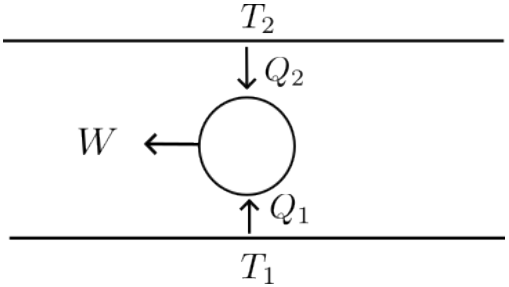
\includegraphics[width=0.4\linewidth]{Immagini/macchina di Carnot 2.png}
    \caption{macchina ciclica reversibile con $T_2 < T_1$.}
    \label{fig: macchina di Carnot 2}
\end{figure}

Combinando le equazioni \eqref{eq: rendimento macchina ciclica reversibile} e \eqref{eq: rendimento macchina ciclica reversibile in funzione di T} si ottiene la disuguaglianza
\begin{equation}
    1 + \frac{Q_1}{Q_2} \le 1 - \frac{T_1}{T_2},
\end{equation}
da cui, se arrangiata opportunamente, si ricava la disuguaglianza di Clausius
\begin{equation}
\label{eq: disuguaglianza di Clausius}
    \frac{Q_1}{T_1} + \frac{Q_2}{T_2} \le 0,
\end{equation}
dove $Q_1 < 0$ per il secondo principio della Termodinamica. La disuguaglianza \eqref{eq: disuguaglianza di Clausius} si può generalizzare ad un numero $n$ di sorgenti con
\begin{equation}
\label{eq: disuguaglianza di Clausius n sorgenti}
    \sum_{i=1}^n\frac{Q_i}{T_i} \le 0,
\end{equation}
e, analogamente, ad un ciclo termodinamico generico, approssimandolo ad una serie di trasformazioni adiabatiche isoterme, con
\begin{equation}
\label{eq: disuguaglianza di Clausius ciclo termodinamico}
    \oint_C\frac{\delta Q}{T} \le 0.
\end{equation}
In particolare, se il ciclo è reversibile, allora
\begin{equation}
\label{eq: disuguaglianza di Clausius ciclo reversibile}
    \oint_C\frac{\delta Q}{T}=0\quad\Rightarrow\quad\frac{\delta Q}{T} = dS,
\end{equation}
dove $dS$ è un differenziale esatto. La funzione di $S$ prende il nome di entropia ed è una funzione di stato, per cui dati due stati diversi $A$ e $B$, la variazione di entropia necessaria per passare da $A$ a $B$ non dipende dal percorso scelto, ossia
\begin{equation}
\label{eq: proprietà funzione di stato entropia}
    \Delta S_{AB} = S_B - S_A.
\end{equation}
Facendo riferimento al ciclo mostrato in figura \ref{fig: ciclo termodinamico generico}, è possibile applicare l'equazione \eqref{eq: disuguaglianza di Clausius ciclo termodinamico} ottenendo
\begin{equation}
    \begin{split}
        \int_A^B\frac{\delta Q_I}{T} + \int_B^A\frac{\delta Q_R}{T} &< 0 \\
        \int_A^B\frac{\delta Q_I}{T} + \int_B^AdS &<0 \\
        \int_A^B\frac{\delta Q_I}{T} + \Delta S_{BA} &< 0 \\
        \int_A^B\frac{\delta Q_I}{T} &< \Delta S_{AB}.
    \end{split}
\end{equation}
Quindi, per un tratto infinitesimo la variazione di entropia è
\begin{equation}
\label{eq: variazione di entropia infinitesima}
    dS = \frac{\delta Q_I}{T} + \delta S_I,\quad \delta S_I > 0,
\end{equation}
dove $\delta S_I$ è la parte di variazione entropica non spiegata dal flusso di calore, legata invece all'aumento del disordine microscopico.
\begin{figure}[h]
    \centering
    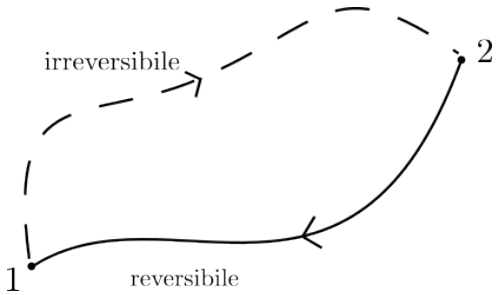
\includegraphics[width=0.4\linewidth]{Immagini/ciclo termodinamico generico.png}
    \caption{ciclo termodinamico generico.}
    \label{fig: ciclo termodinamico generico}
\end{figure}

In particolare, per processi spontanei, ovvero adiabatici (con $\delta Q = 0$) e irreversibili, la variazione di entropia è
\begin{equation}
    dS = \delta S_I > 0,
\end{equation}
una relazione equivalente al secondo principio della Termodinamica. Inoltre, dire che uno stato di equilibrio è stabile rispetto a fluttuazioni spontanee equivale a dire che coincide con un massimo dell'entropia. Una proprietà importante dell'entropia è l'essere estensiva, essendo una funzione dipendente dal calore $Q$, estensivo, e dalla temperatura $T$, intensiva. Combinando le equazioni \eqref{eq: combinazione espressione lavoro e I PDT} e \eqref{eq: disuguaglianza di Clausius} si ottiene
\begin{equation}
\label{eq: disuguaglianza tra TdS e dE}
    TdS \ge dE + pdV -\mu dN - ydx,
\end{equation}
dove il caso di uguaglianza si presenta se il ciclo è reversibile e vale \eqref{eq: disuguaglianza di Clausius ciclo reversibile}. 

Ad ogni modo, l'entropia si dice essere una funzione estensiva di variabili estensive\footnote{Per semplicità si evita spesso di evidenziare la dipendenza dagli spostamenti generalizzati $X$.}, effettivamente $S \equiv S(E,V,N,X)$. Quindi, conoscere $S$ equivale a conoscere le equazioni di stato, infatti
\begin{align}
\label{eq: equazioni di stato da S}
    \frac{\p S}{\p E}\bigg|_{V,N,X}&=\frac{1}{T},\quad\mathrm{(equazione\,di\,stato\,termica)}, \\
    \frac{\p S}{\p N}\bigg|_{E,V,X}&=-\frac{\mu}{T},\quad\mathrm{(equazione\,di\,stato\,chimica)}, \\
    \frac{\p S}{\p V}\bigg|_{E,N,X}&=\frac{p}{T},\quad\mathrm{(equazione\,di\,stato\,meccanica)}, \\
    \frac{\p S}{\p X}\bigg|_{E,V,N}&=-\frac{y}{T},\quad\mathrm{(equazione\,di\,stato\,generalizzata)}.
\end{align}
\begin{obs}
    In Termodinamica, le espressioni delle equazioni di stato sono ricavate ``sperimentalmente'' e da esse si ricava l'espressione di $S(E,V,N,X)$. Invece, in Meccanica statistica si deriva prima $S(E,V,N,X)$ per poi derivare le equazioni \eqref{eq: equazioni di stato da S}. 
\end{obs}
La caratteristica dell'entropia di funzione estensiva di variabili estensive implica che se si scalano le grandezze da cui $S$ dipende di un fattore reale $\lambda$ si ha
\begin{equation}
\label{eq: S funzione omogenea di I grado}
    S(\lambda E,\lambda V,\lambda N,\lambda X) = \lambda S(E,V,N,X),\quad \lambda\in\R^+.
\end{equation}
L'equazione \eqref{eq: S funzione omogenea di I grado} implica che $S$ è una funzione omogenea di primo grado\footnote{In generale, una funzione $f(x_i)$ si dice omogenea di grado $d$ se soddisfa la relazione $f(\lambda x_i) = \lambda^d f(x_i)$ e se è autofunzione dell'operatore di Eulero $D=\nsum_ix^i\p_{x_i}$, ossia se $Df(x_i)=df(x_i)$.} nelle sue variabili. Dunque, nel caso dell'entropia si ha
\begin{multline}
    S = E\bigg(\frac{\p S}{\p E}\bigg|_{V,N,X}\bigg) + V\bigg(\frac{\p S}{\p V}\bigg|_{E,N,X}\bigg) + \\
    + N\bigg(\frac{\p S}{\p N}\bigg|_{E,V,X}\bigg) + X\bigg(\frac{\p S}{\p X}\bigg|_{E,V,N}\bigg),
\end{multline}
che, se si sostituiscono le equazioni \eqref{eq: equazioni di stato da S} e si moltiplica per $T$, si ricava l'equazione fondamentale della Termodinamica
\begin{equation}
\label{eq: equazioni fondamentale della TD}
    TS = E + pV - \mu N - yX.
\end{equation}
\begin{obs}
    L'equazione \eqref{eq: equazioni fondamentale della TD} potrebbe sembrare l'integrale ``sbagliato'' dell'equazione \eqref{eq: disuguaglianza tra TdS e dE}, ma in realtà è corretto dato che $S$ è una funzione omogenea di primo grado.    
\end{obs}
Differenziando l'equazione \eqref{eq: equazioni fondamentale della TD} e sostituendo la \eqref{eq: disuguaglianza tra TdS e dE} nel caso reversibile si ottiene l'equazione di Gibbs-Duhem
\begin{equation}
\label{eq: equazione di Gibbs-Duhem}
    SdT = Vdp - Nd\mu - Xdy.
\end{equation}
Invertendo $S(E,V,N,X)$ si può vedere l'energia $E$ come funzione di variabili estensive $E\equiv E(S,V,N,X)$, dall'equazione di stato termica in \eqref{eq: equazioni di stato da S} segue che
\begin{equation}
    \frac{\p E}{\p S}\bigg|_{V,N,X}=T.
\end{equation}
Ricordando la relazione \eqref{eq: disuguaglianza tra TdS e dE} si deduce che per sistemi chiusi, ovvero tali che $dN = 0$, a cui non viene fornito calore in modo reversibile, ovvero $dS = 0$, isocoro, ovvero con $dV = 0$, e con tutte le altri variabili estensive fisse, ovvero $dX = 0$, per ogni trasformazione si ha 
\begin{equation}
    dE \le 0,
\end{equation}
per cui il sistema evolve verso uno stato di equilibrio coincidente con un minimo di energia. L'energia interna $E$ gioca dunque un ruolo analogo all'energia potenziale in Meccanica quando le variabili di controllo del sistema sono $\{S,V,N,X\}$. In tal caso, le funzioni estensive come l'energia $E$ sono funzioni omogenee di primo grado e quindi
\begin{equation}
\label{eq: equazioni di stato da E}
    \begin{split}
         T=\frac{\p E}{\p S}\bigg|_{V,N,X}&,\quad p=-\frac{\p E}{\p V}\bigg|_{S,N,X}, \\
         \mu=\frac{\p E}{\p N}\bigg|_{S,V,X}&,\quad y=\frac{\p E}{\p X}\bigg|_{S,V,N},
    \end{split}
\end{equation}
che sono funzioni omogenee di grado zero come è evidente da queste relazioni, ad esempio
\begin{equation}
    p(\lambda S,\lambda V,\lambda N,\lambda X) = p(S,V,N,X),\quad\lambda\in\R^+.
\end{equation}
In particolare, scegliendo $\lambda = 1/N$ si ha 
\begin{equation}
    p(\lambda S,\lambda V,\lambda N,\lambda X) = p(s,v,n,x) \equiv p(s,v,x),
\end{equation}
dove $s = S/N$, $v = V/N$ e $x = X/N$ sono l'entropia, il volume e lo spostamento generalizzato della singola componente. Se quindi si hanno $3 + r$ variabili estensive indipendenti quali $S$, $V$, $N$ e gli $r$ spostamenti $X$, le grandezze intensive a loro coniugate sono solo $2 + r$ rapporti indipendenti di tali variabili.

Potrebbe essere conveniente usare un insieme di variabili di controllo che contengono alcune delle variabili intensive $T$, $p$, $\mu$ e $y$, che in termini di $E$ sono espresse dalle equazioni \eqref{eq: equazioni di stato da E}. La tecnica matematica necessaria per passare dalle variabili estensive alle loro coniugate intensive è la trasformata di Legendre\footnote{\'E la stessa trasformata che viene applicata per passare dalla descrizione lagrangiana a quella hamiltoniana.}. In questo modo si definiscono altri potenziali termodinamici adatti a diversi insiemi di variabili di controllo. 

\paragraph{Energia libera di Helmoltz.} Applicando la trasformata di Legendre rispetto alla coppia di variabili $(T=\p_S E,S)$ si ottiene
\begin{equation}
\label{eq: TdL rispetto a (T,S)}
    F(T,V,N,X) = E(S,V,N,X) - TS,
\end{equation}
dove nel secondo membro $S$ è pensata come dipendente ed ottenuta invertendo la relazione $T=\p_S E$. Usando l'equazione fondamentale \eqref{eq: equazioni fondamentale della TD} si può scrivere
\begin{equation}
\label{eq: espressione di F}
    F = -pV + \mu N + yX.
\end{equation}
Ora differenziando l'equazione \eqref{eq: TdL rispetto a (T,S)} e tenendo conto della \eqref{eq: disuguaglianza tra TdS e dE} si ottiene
\begin{equation}
    dF \le -SdT -pdV + \mu dN + ydX.
\end{equation}
Per un sistema chiuso ($dN = 0$), a temperatura costante ($dT = 0$), a volume costante ($dV = 0$) e con tutte le altre variabili estensive fisse ($dX = 0$), per ogni trasformazione si ha
\begin{equation}
    dF \le 0,
\end{equation}
per cui il sistema evolve verso uno stato di equilibrio coincidente con un minimo di $F$ che prende il nome di energia libera di Helmoltz. Le variabili dipendenti in questo caso sono 
\begin{equation}
\label{eq: equazioni di stato da F}
    \begin{split}
        S = -\frac{\p F}{\p T}\bigg|_{V,N,X}&,\quad p = -\frac{\p F}{\p V}\bigg|_{T,N,X}, \\
        \mu = \frac{\p F}{\p N}\bigg|_{T,V,X}&,\quad y = \frac{\p F}{\p X}\bigg|_{T,V,N}.
    \end{split}
\end{equation}
\paragraph{Entalpia.} Applicando la trasformata di Legendre alla coppia di variabili $(p = -\p_V E,V)$ si ottiene
\begin{equation}
\label{eq: TdL rispetto a (p,V)}
    H(S,p,N,X) = E(S,V,N,X) + pV,
\end{equation}
dove nel secondo membro $V$ è pensato come dipendente ed ottenuto invertendo l'equazione di stato meccanica $p = -\p_V E$. Usando l'equazione fondamentale \eqref{eq: equazioni fondamentale della TD} si può scrivere 
\begin{equation}
\label{eq: espressione di H}
    H = TS + \mu N + yX.
\end{equation}
Ora differenziando l'equazione \eqref{eq: TdL rispetto a (p,V)} e tenendo conto della \eqref{eq: disuguaglianza tra TdS e dE} si ottiene
\begin{equation}
    dH \le TdS + Vdp +\mu dN +ydX.
\end{equation}
Per un sistema chiuso ($dN = 0$), in condizioni isoentorpiche ($dS = 0$), ossia senza trasferimento reversibile di calore, a pressione costante ($dp = 0$) e con tutte le altre variabili estensive fisse ($dX = 0$), per ogni trasformazione si ha
\begin{equation}
    dH \le 0,
\end{equation}
per cui il sistema evolve verso uno stato di equilibrio coincidente con un minimo di $H$ che prende il nome di entalpia. Le variabili dipendenti in questo caso sono 
\begin{equation}
\label{eq: equazioni di stato da H}
    \begin{split}
        T = \frac{\p H}{\p S}\bigg|_{p,N,X}&,\quad V = \frac{\p H}{\p p}\bigg|_{S,N,X}, \\
        \mu = \frac{\p H}{\p N}\bigg|_{S,p,X}&,\quad y = \frac{\p H}{\p X}\bigg|_{S,p,N}.
    \end{split}
\end{equation}

\paragraph{Energia libera di Gibbs.} Applicando la trasformata di Legendre sia alla coppia di variabili $(-p,V)$ che alla coppia $(T,S)$ si ottiene
\begin{equation}
\label{eq: TdL rispetto a (-p,V) e a (T,S)}
    G(T,p,N,X) = E(S,V,N,X) - TS +pV,
\end{equation}
dove $S$ e $V$ sono pensate come dipendenti ed ottenute invertendo le equazioni di stato rispettive tra le \eqref{eq: equazioni di stato da E}. Usando l'equazione fondamentale \eqref{eq: equazioni fondamentale della TD} si può riscrivere
\begin{equation}
\label{eq: espressione di G}
    G = \mu N + yX,
\end{equation}
che si riduce a $G = \mu N$ se nel sistema non compaiono variabili $(y,X)$. Differenziando la \eqref{eq: TdL rispetto a (-p,V) e a (T,S)} e tenendo conto della \eqref{eq: disuguaglianza tra TdS e dE} si ottiene
\begin{equation}
    dG \le -SdT + Vdp +\mu dN +ydX.
\end{equation}
Per un sistema chiuso ($dN = 0$), a pressione costante ($dp = 0$), a temperatura costante ($dT = 0$) e con tutte le altre variabili estensive fisse ($dX = 0$), per ogni trasformazione si ha
\begin{equation}
    dG \le 0,
\end{equation}
per cui ogni sistema evolve verso uno stato di equilibrio coincidente con un minimo di $G$ che prende il nome di energia libera di Gibbs. Le variabili dipendenti in questo caso sono
\begin{equation}
\label{eq: equazioni di stato da G}
    \begin{split}
        S = -\frac{\p G}{\p T}\bigg|_{p,N,X}&,\quad V = \frac{\p G}{\p p}\bigg|_{T,N,X}, \\
        \mu = \frac{\p G}{\p N}\bigg|_{T,p,X}&,\quad y = \frac{\p G}{\p X}\bigg|_{T,p,N}.
    \end{split}
\end{equation}

\paragraph{Potenziale grancanonico.} Applicando la trasformata di Legendre sia alla coppia di variabili $(T,S)$ che alla coppia $(\mu,N)$ si ottiene
\begin{equation}
\label{eq: TdL rispetto a (T,S) e (mu,N)}
    \varpi(T,V,\mu,X) = E(S,V,N,X) - TS - \mu N,
\end{equation}
dove $S$ ed $N$ sono pensate come indipendenti ed ottenute invertendo le equazioni di stato rispettive tra le \eqref{eq: equazioni di stato da E}. Usando l'equazione fondamentale \eqref{eq: equazioni fondamentale della TD} si può riscrivere 
\begin{equation}
\label{eq: espressione del pot. grancanonico}
    \varpi = -pV + yX,
\end{equation}
che si riduce a $\varpi =  -pV$ se nel sistema non compaiono variabili $(y,X)$. Differenziando la \eqref{eq: TdL rispetto a (T,S) e (mu,N)} e tenendo conto della \eqref{eq: disuguaglianza tra TdS e dE} si ottiene
\begin{equation}
    d\varpi \le -SdT -pdV - N\mu +ydX.
\end{equation}
Per un sistema aperto, ma a potenziale chimico costante ($d\mu = 0$), a temperatura costante ($dT = 0$), in condizioni isobariche ($dV = 0$) e con tutte le altr variabili estensive fisse ($dX = 0$), per ogni trasformazioni si ha
\begin{equation}
    d\varpi \le 0,
\end{equation}
per cui ogni sistema evolve verso uno stato di equilibrio coincidente con un minimo di $\varpi$ che prende il nome di potenziale grancanonico. Le variabili indipendenti in questo caso sono
\begin{equation}
\label{eq: equazioni di stato dapot. grancanonico}
    \begin{split}
        S = -\frac{\p \varpi}{\p T}\bigg|_{V,\mu,X}&,\quad p = -\frac{\p \varpi}{\p V}\bigg|_{T,\mu,X}, \\
        N = \frac{\p \varpi}{\p \mu}\bigg|_{T,V,X}&,\quad y = \frac{\p \varpi}{\p X}\bigg|_{T,V,\mu}.
    \end{split}
\end{equation}

\paragraph{Potenziali generali.} In linea di principio è possibile ottenere, a partire dai precedenti, ulteriori potenziali applicando la trasformata di Legendre rispetto alle coppie, alcune o tutte, di variabili $(y,X)$. Per tali potenziali non esistono nomi specifici; tuttavia, possono essere quelli convenienti in date situazioni in cui le variabili tra le di controllo compaiono alcune delle $y$. In particolare, se a partire da $G$ si applica la trasformata di Legendre rispetto a tutte le coppie $(y,X)$ si ottiene
\begin{equation}
    \tilde{G}(T,p,N,y) = G(T,p,N,X) -yX,
\end{equation}
dove $X$ è vista come indipendente ottenuta invertendo la relazione rispettiva tra le \eqref{eq: equazioni di stato da G}. Dalla \eqref{eq: espressione di G} segue che 
\begin{equation}
    \tilde{G} = \mu N,
\end{equation}
e quindi il potenziale specifico $\tilde{g} = \tilde{G}/N$ coincide proprio con il potenziale chimico $\mu$. Allo stesso modo si può ragionare per $\varpi$ ottenendo 
\begin{equation}
    \tilde{\varpi}(T,V,\mu,y) = \varpi(T,V,\mu,X) - yX
\end{equation}
e dalla \eqref{eq: espressione del pot. grancanonico} segue che
\begin{equation}
    \tilde{\varpi} = -pV
\end{equation}
e quindi la densità di potenziale $\tilde{\varpi}/V$ coincide con $-p$.

\section{Funzioni di risposta} 
Le funzioni di risposta sono quantità che descrivono come una data funzione di stato cambi al variare di un'altra variabili indipendente in condizioni controllate; in particolare, è interessante il caso in cui le due variabili sono coniugate. Inoltre, sono le quantità più direttamente misurabili sperimentalmente. Sono legate poi, dal punto di vista macroscopico, alla grandezza delle fluttuazioni del sistema. Le funzioni di risposta si dividono in due grandi categorie: termiche e meccaniche. Si considerano nel seguito alcune delle più importanti.

\subsubsection{Capacità termica}
La capacità termica misura la quantità di calore che è necessario fornire ad un sistema per variarne la temperatura di una quantità fissata, per cui la definizione generale è
\begin{equation}
    c = \frac{\delta Q}{dT}.
\end{equation}
Dato che $\delta Q$ non è un differenziale è necessario specificare il tipo di trasformazione con cui il calore viene fornito.

Se $\delta W = pdV - \mu dN - ydX  = 0$, allora dal primo principio della Termodinamica si ha $\delta Q = dE$, per cui si definisce la capacità termica a volume costante $c_V$ come
\begin{equation}
\label{eq: capacità termica V costante}
    c_{V,N,X} \equiv c_V = \frac{\p E}{\p T}\bigg|_{V,N,X}.
\end{equation}
Si può esprimere \eqref{eq: capacità termica V costante} anche in funzione dell'entropia usando $\delta Q = TdS$; se questo è il caso, allora si stanno usando come variabili indipendenti $\{T,V,N.X\}$ le cui ultime tre sono fisse, per cui 
\begin{equation}
    dS = \frac{\p S}{\p T}\bigg|_{V,N,X}dT
\end{equation}
e quindi
\begin{equation}
    c_V = T\frac{dS}{dT} = T\frac{\p S}{\p T}\bigg|_{V,N,X}.
\end{equation}
Avendo come variabili indipendenti $\{T,V,N,X\}$ il potenziale rilevante è l'energia libera di Helmoltz $F(T,V,N,X)$ e l'entropia è vista come
\begin{equation}
    S = -\frac{\p F}{\p T}\bigg|_{V,N,X},
\end{equation}
quindi si può scrivere
\begin{equation}
    c_V = -T\frac{\p^2F}{\p T^2}\bigg|_{V,N,X}
\end{equation}

Se invece $\delta W = pdV$, allora sempre dal primo principio della Termodinamica si ha $\delta Q = dE + pdV$, per cui si definisce al capacità termica a pressione costante $c_p$ come 
\begin{equation}
\label{eq: capacità termica p costante}
    c_{p,V,X} \equiv c_p = \frac{\p E}{\p T}\bigg|_{p,N,X} + p\frac{\p V}{\p T}\bigg|_{p,N,X}.
\end{equation}
Avendo come variabili di indipendenti $\{T,p,N,X\}$ il potenziale rilevante è l'energia libera di Gibbs $G(T,p,N,X)$ e l'energia è vista come
\begin{equation}
    E = G + TS -pV = G - T\frac{\p G}{\p T} - pV,
\end{equation}
dove si sono usate le relazioni \eqref{eq: equazioni di stato da G}, che sostituita nella \eqref{eq: capacità termica p costante} restituisce
\begin{equation}
    \begin{split}
        c_p &= \frac{\p}{\p T}\bigg(G - T\frac{\p G}{\p T} - pV\bigg)\bigg|_{p,N,X} + p\frac{\p V}{\p T}\bigg|_{p,N,X} \\
        &=\bigg(\frac{\p G}{\p T} - \frac{\p G}{\p T} -T\frac{\p^2G}{\p T^2}\bigg)\bigg|_{p,N,X} \\
        &=-T\frac{\p^2 G}{\p T^2}\bigg|_{p,N,X}.
    \end{split}
\end{equation}
Il medesimo risultato si può ottenere a partire da $\delta Q = TdS$.

\subsubsection{Suscettività termica}
La suscettività di un sistema indica di quanto il volume aumenta al crescere delle pressione. Dato che ciò può essere effettuato in modi diversi è necessario specificare il tipo di trasformazione, in particolare indicando quali variabili vengono mantenute costanti.

Se si mantengono costanti le variabili $\{T,N,X\}$, allora si definisce la suscettività isoterma $\chi_T$ come
\begin{equation}
    \chi_T = -\frac{\p V}{\p p}\bigg|_{T,N,X}.
\end{equation}
Se le variabili indipendenti sono $\{T,p,N,X\}$, allora il potenziale rilevante è l'energia libera di Gibbs $G$, per cui esprimendo $V$ tramite l'equazione rispettiva tra le \eqref{eq: equazioni di stato da G} si ha
\begin{equation}
    \chi_T = -\frac{\p^2 G}{\p p^2}\bigg|_{T,N,X}. 
\end{equation}

Se invece si mantengono costanti le variabili $\{S,N,X\}$, allora si definisce la suscettività adiabatica come
\begin{equation}
    \chi_S = -\frac{\p V}{\p p}\bigg|_{S,N,X}.
\end{equation}
Se le variabili indipendenti sono $\{S,p,N,X\}$, allora il potenziale rilevante è l'entalpia $H$, per cui esprimendo $V$ tramite l'equazione rispettiva tra le \eqref{eq: equazioni di stato da H} si ha
\begin{equation}
    \chi_S = -\frac{\p^2 H}{\p p^2}\bigg|_{S,N,X}.
\end{equation}

\subsubsection{Compressibilità termica}
La compressibilità di un sistema esprime la variazione percentuale di volume in seguito ad un cambiamento di pressione.

Se la variazione di pressione avviene mantenendo la temperatura $T$ costante, allora si definisce la compressibilità isoterma $\kappa_T$ come
\begin{equation}
    \kappa_T = \frac{\chi_T}{V} = -\frac{1}{V}\frac{\p^2 G}{\p p^2}\bigg|_{T,N,X}.
\end{equation}

Se invece la variazione di pressione avviene mantenendo l'entropia $S$ costante, allora si definisce la compressibilità adiabatica come 
\begin{equation}
    \kappa_S = \frac{\chi_S}{V} = -\frac{1}{V}\frac{\p^2 H}{\p p^2}\bigg|_{S,N,X}
\end{equation}

\subsubsection{Espansibilità termica}
L'espansibilità termica descrive il cambiamento di volume in funzione della temperatura mantenendo costanti le variabili $\{p,N,X\}$, definita da
\begin{equation}
    \alpha_{p,N,X} \equiv \alpha_p = \frac{\p V}{\p T}\bigg|_{p,N,X}.
\end{equation}
In questo caso $V$ e $T$ non sono variabili coniugate, quindi $\alpha_p$ è collegata ad una derivata seconda mista del potenziale $G(T,p,N,X)$, infatti esprimendo $V$ con l'equazione rispettiva tra le \eqref{eq: equazioni di stato da G} si ha
\begin{equation}
    \alpha_p = \frac{\p^2 G}{\p p\p T}\bigg|_{N,X}.
\end{equation}

\section{Relazioni tra variabili}
In Termodinamica si ha continuamente a che fare con funzioni di molteplici variabili e con differenti scelte di set di variabili. Alcune identità matematiche forniscono delle relazioni utili per svariate grandezze termodinamiche.

Innanzitutto, l'ordine della derivazione parziale di una funzione non conta, ossia
\begin{equation}
\label{eq: ordine derivate parziali irrilevante}
    \frac{\p^2 f}{\p x^i\p x^j} = \frac{\p^2 f}{\p x^j \p x^i},
\end{equation}
e questo si estende a derivate parziali di ordine superiore. Si considerino ora tre variabili $x$, $y$ e $z$ legate da una relazione del tipo $f(x,y,z) = 0$, per cui si può scegliere arbitrariamente due di esse come indipendenti. In questo modo, si hanno
\begin{equation}
    \frac{\p x}{\p y}\bigg|_z = \bigg(\frac{\p y}{\p x}\bigg|_z\bigg)^{-1},\quad\frac{\p x}{\p y}\bigg|_z\frac{\p y}{\p z}\bigg|_x\frac{\p z}{\p x}\bigg|_y = -1.
\end{equation}
Si consideri un'ulteriore funzione $w\equiv w(x,y,z)$ con due delle variabili da cui dipende sempre scelte arbitrariamente indipendenti, così si hanno
\begin{equation}
    \frac{\p x}{\p w}\bigg|_z = \frac{\p x}{\p y}\bigg|_z\frac{\p y}{\p w}\bigg|_z,\quad\frac{\p x}{\p y}\bigg|_z = \frac{\p x}{\p y}\bigg|_w + \frac{\p x}{\p w}\bigg|_y\frac{\p w}{\p y}\bigg|_z.
\end{equation}

A partire dalle equazioni di stato \eqref{eq: equazioni di stato da E} che definiscono le variabili intensive in termini di $E$, usando la \eqref{eq: ordine derivate parziali irrilevante}, si ha
\begin{equation}
    \frac{\p T}{\p V}\bigg|_{S,N,X} = \frac{\p^2 E}{\p V\p S}\bigg|_{N,X} = \frac{\p}{\p S}\bigg(\frac{\p E}{\p V}\bigg|_{N,X}\bigg) = -\frac{\p p}{\p S}\bigg|_{V,N,X}.
\end{equation}
In modo analogo, si hanno
\begin{align}
    \frac{\p T}{\p N}\bigg|_{S,V,X} &= \frac{\p^2 E}{\p N\p S}\bigg|_{N,X} = \frac{\p\mu}{\p S}\bigg|_{N,X}, \\
    \frac{\p T}{\p X}\bigg|_{S,V,N} &= \frac{\p^2 E}{\p X\p S}\bigg|_{V,N} = \frac{\p y}{\p S}\bigg|_{V,N,X}, \\
    \frac{\p p}{\p N}\bigg|_{S,V,X} &= -\frac{\p^2 E}{\p N\p V}\bigg|_{S,X} = -\frac{\p \mu}{\p V}\bigg|_{S,V,X}, \\
    \frac{\p p}{\p X}\bigg|_{S,V,N} &= -\frac{\p^2 E}{\p X\p V}\bigg|_{S,X} = -\frac{\p y}{\p V}\bigg|_{S,N,X}, \\
    \frac{\p \mu}{\p X}\bigg|_{S,N,V} &= \frac{\p^2 E}{\p X\p N}\bigg|_{S,V} = \frac{\p y}{\p N}\bigg|_{S,V,X}.
\end{align}
Analoghe relazioni si possono trovare a partire dagli altri potenziali termodinamici, cioè da altri set di  variabili indipendenti. La regola generale è la seguente. Se $\{z_i\}$ è l'insieme di variabili indipendenti scelto e $\{\zeta_i\}$ sono le variabili coniugate, in modo che il potenziale appropriato sia
\begin{equation}
    d\Phi = \nsum_i\zeta_idz_i,
\end{equation}
allora
\begin{equation}
    \frac{\p\zeta_A}{\p z_B}\bigg|_{\{z_i\}\setminus z_B} = \frac{\p^2\Phi}{\p z_B \p z_A}\bigg|_{\{z_i\}\setminus \{z_B,z_A\}} = \frac{\p \zeta_B}{\p z_A}\bigg|_{\{z_i\}\setminus z_B}.
\end{equation}

A partire dalle definizioni \eqref{eq: capacità termica V costante} e \eqref{eq: capacità termica p costante} si possono usare le identità matematiche elencate per ricavare una relazione tra $c_V$, $c_p$, $\chi_T$ e $\alpha_p$; questa è
\begin{equation}
    c_p = c_V + \frac{T}{\chi_T}\alpha_p^2.
\end{equation}



